\externaldocument{modelling}

\section{Method}

%insert correct equation labels, figure refrences
%insert correct citataions
%correct systematic variation table
%insert initial values figure.

This work will investigate how the free parameters of the model given by the equations \ref{eq:6}-\ref{eq:10} will affect the spatial temporal progress of the numerical simulation. For the numerical simulation we will use the weak form given with equations \ref{eq:11} - \ref{eq:13} and solve it using HiFlow. To study the results of the numerical simulation ParaView is used, producing informative plots to compare the evolution of the simulation in time. For this we rely on the tool Plot Over Line to give radially symmetrical reulsts of the three variables of tumour and extracellular matrix density and matrix-degrading enzymes, like seen in the inital distribution in figure , in figure you can see the configuraion for the Plot Over Line tool used, the grey line in the middle of the simulation to the middle of the top of the square.\newline
\begin{figure}
    \centering
    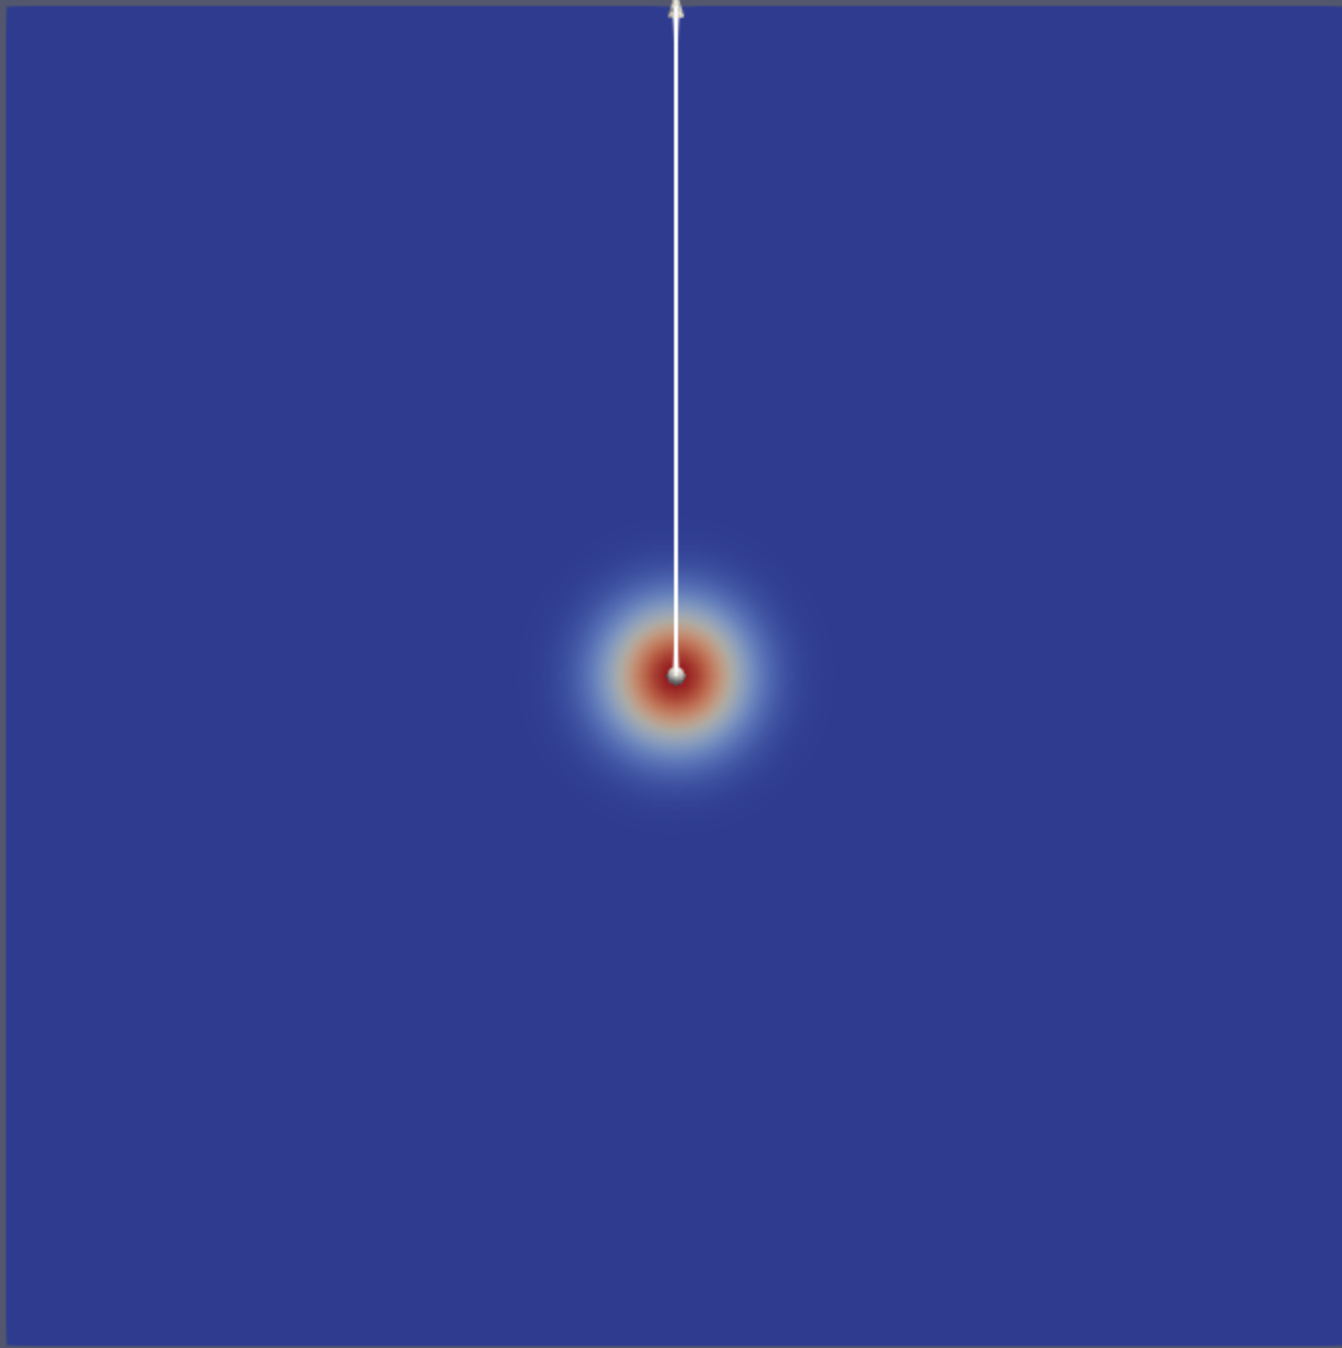
\includegraphics[width=0.3\textwidth]{resources/images/plot_over_line_tool.png}
    \caption{Plot Over Line Tool Configuration}
    \label{fig:PlotOverLine}
\end{figure}
All experiments, except when introducing the heterogenous ECM, start with the same initial values as seen in figuer initial values.\newline 
First replications of simulations of previous works will be discussed whhich serves the purpose to first verify the correctness of our result, as well as to give a starting point describing the phenomena this model exhibits. We start with the 2D case, since for this there are many examples already given and then move on to 3D simulation where the examples are fewer. \newline
After having taken a look at the preexisting experiments the main part of this work will begin with a systematic parameter analysis. Like before it will start investigating 2D simulation and will then move on to 3D simulation. Here we will also compare what effect the dimensionality has on the simulation, for example of the amount of overall values for $c,e,m$ and try replicating the behaviour of the 2D cases in the 3D variant. \newline
At last we will have a prospect on how an heterogneous extracellular matrix influences the results, which is the more realistic case, since tumourous cells tend to appear at border regions of tissue where we do not have a homogenous ECM, like it is rather found inside a tissue region. \newline
The results of the above experiments will be summarized and discussed in the Conclusion and Discussion part, pointing out the important characteristics of the simulation and disucssing the sensitivity of each of the parameters. At this point we will have an outlook on how to extend the model in more continuous and or discrete adaptations.
Looking at these estimates of section 3 we are left with plenty of room to investigate the effects of every single parameter. For this systematic analysis we are going to assume a baseline set of parameters, $(d_c, \gamma, \mu_1, \eta, \mu_2, d_m, \alpha, \beta) = (0.001, 0.005, 0, 10, 0, 0.001,0.1, 0)$ for experiments without proliferation and \newline
$(d_c, \gamma, \mu_1, \eta, \mu_2, d_m, \alpha, \beta) = (0.001, 0.005, 0.3, 10, 0.3, 0.001,0.1, 0.1)$ for experiments with proliferation, where in every experiment one paramter will be changed. Later this will be extended to study a cross-analysis, where more than one parameter is changed at a time. The set of baseline parameters is taken from previous experiments done by Anderson et. al \cite{anderson_mathematical_2000} and Kolev et al.\cite{Kolev2010}. The systematic variations will be same for 2D as well as 3D experiments and can be found in talbe \ref{tab:systematic_analysis}.

\begin{table}[!h]
    \begin{center}
        \label{tab:systematic_analysis}
        \begin{tabular}{||c c c c||} 
            \hline
            Col1 & Col2 & Col2 & Col3 \\ [0.5ex] 
            \hline\hline
            1 & 6 & 87837 & 787 \\ 
            \hline
            2 & 7 & 78 & 5415 \\
            \hline
            3 & 545 & 778 & 7507 \\
            \hline
            4 & 545 & 18744 & 7560 \\
            \hline
            5 & 88 & 788 & 6344 \\ [1ex] 
            \hline
        \end{tabular}
        \caption{Your caption.}
    \end{center}
\end{table}

\begin{comment}

\subsection{Software and Implementation}
\subsection{Systematic Parameter Analysis}
\subsubsection{2D}
\subsubsection{3D}
\subsubsection{Non-heterogenous ECM Structure}

This work will investigate how the results of the modified model in the modelling section will be affected be varying free parameters $\lambda, \delta, \mu_1, \mu_2, \mu_3$ as well as how the chosen dimension for a simulation will influence the output.
For this we will start with comparing results first within the same dimension, varying the free parameters. Conducting these experiments we hope that we can see a pattern occuring, which is shared across one dimension. After this we will investigate how the results are changed when we change the dimension but keep the free parameters the same. 


\begin{center}
\begin{tabular}{|| c | c | c | c | c || c | c | c | c | c || c | c | c | c | c ||}
    \hhline{||=|=|=|=|=||=|=|=|=|=||=|=|=|=|=||}
    1D \small & & & & & 2D & & & & & 3D & & & & \\
    \hhline{||=|=|=|=|=||=|=|=|=|=||=|=|=|=|=||}
    $\lambda$ & $\delta$ & $\mu_1$ & $\mu_2$ & $\mu_3$  & $\lambda$ & $\delta$ & $\mu_1$ & $\mu_2$ & $\mu_3$ & $\lambda$ & $\delta$ & $\mu_1$ & $\mu_2$ & $\mu_3$ \\ 
    \hline
    a & b & c & d & e & a & b & c & d & e & a & b & c & d & e \\ \hline 
    a & b & c & d & e & a & b & c & d & e & a & b & c & d & e \\ \hline 
    a & b & c & d & e & a & b & c & d & e & a & b & c & d & e \\ \hline 
    a & b & c & d & e & a & b & c & d & e & a & b & c & d & e \\ \hhline{||=|=|=|=|=||=|=|=|=|=||=|=|=|=|=||} 

\end{tabular}
\end{center}

When comparing the effects of the free parameters on the simulation we need to keep in mind, that some of them are by assupmtion fixed, whilst others are defined within a reasonable range and again others have no restrictions at all, for those we assume the value ranges in the modelling section. At this first stage of the investigation we change only one parameter within each group of experiments, for example we only study how the output changes when $\delta$ changes, we do this with every parameter and compare the results within their dimension. When we are done with that we compare the results with changing dimension whilst keeping every other free parameter equal. \newline
With the core question that if different dimensions yield different results, we hope to find characteristics prevailing in each dimension, but mainly concentrate on the features that arise with the same choice of parameters varying the dimension. We hope to find answers to which changes in outcome emerge and how to explain the different results. \newline
As a last step this work compares the found results with clinical results, from in-vitro results. Why in-vitro, because this models lacks the biological complexity which governs many effects regarding tumor growth in living bodies, which would yield to quite different behaviour.
\end{comment}